
\begin{figure}
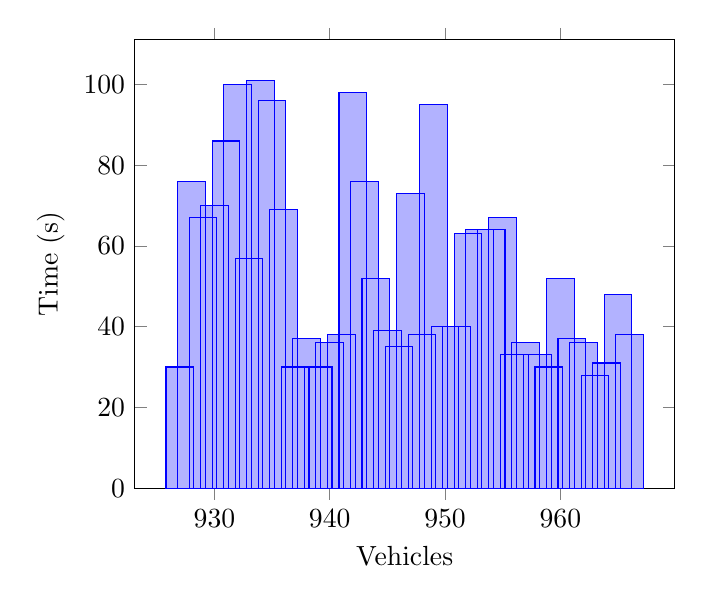
\begin{tikzpicture}
\begin{axis}[
legend style={anchor=west},
xlabel=Vehicles,
ylabel=Time (s),
ymin=0,
ybar,
]
\addplot coordinates {
(948, 38)
(949, 95)
(946, 35)
(947, 73)
(944, 52)
(945, 39)
(942, 98)
(943, 76)
(940, 36)
(941, 38)
(938, 37)
(933, 57)
(932, 100)
(931, 86)
(930, 70)
(937, 30)
(936, 69)
(934, 101)
(929, 67)
(927, 30)
(950, 40)
(928, 76)
(952, 63)
(939, 30)
(964, 31)
(965, 48)
(966, 38)
(960, 52)
(961, 37)
(962, 36)
(963, 28)
(951, 40)
(956, 33)
(935, 96)
(959, 30)
(958, 33)
(953, 64)
(955, 67)
(954, 64)
(957, 36)
};

\end{axis}
\end{tikzpicture}
\label{tik:time:100:11}
\caption{100 percent diving with GSC on route $11$}
\end{figure}
